%%% start preambling . . .  %%%
\documentclass{article}

% required 
\usepackage{rotating}
\usepackage{color}
\usepackage{tabularray}
\usepackage{amsmath}
\usepackage{array}
\usepackage{natbib}
\usepackage{xr-hyper}
\usepackage{hyperref}
\externaldocument[manuscript-]{manuscript}
\usepackage{booktabs,siunitx}
\usepackage{Sweave}
\usepackage{graphicx}
\usepackage{lipsum}                     % Dummytext % https://tex.stackexchange.com/questions/9796/how-to-add-todo-notes
\usepackage{xargs}                      % Use more than one optional parameter in a new commands
\usepackage[pdftex,dvipsnames]{xcolor}  % Coloured text etc.

\usepackage[colorinlistoftodos,prependcaption,textsize=tiny]{todonotes}
\newcommandx{\unsure}[2][1=]{\todo[linecolor=red,backgroundcolor=red!25,bordercolor=red,#1]{#2}}
\newcommandx{\change}[2][1=]{\todo[linecolor=blue,backgroundcolor=blue!25,bordercolor=blue,#1]{#2}}
\newcommandx{\info}[2][1=]{\todo[linecolor=OliveGreen,backgroundcolor=OliveGreen!25,bordercolor=OliveGreen,#1]{#2}}
\newcommandx{\improvement}[2][1=]{\todo[linecolor=Plum,backgroundcolor=Plum!25,bordercolor=Plum,#1]{#2}}
\newcommandx{\thiswillnotshow}[2][1=]{\todo[disable,#1]{#2}}


% https://tex.stackexchange.com/questions/60209/how-to-add-an-extra-level-of-sections-with-headings-below-subsubsection
\usepackage{titlesec}
\setcounter{secnumdepth}{4}

\titleformat{\paragraph}
{\normalfont\normalsize\bfseries}{\theparagraph}{1em}{}
\titlespacing*{\paragraph}
{0pt}{3.25ex plus 1ex minus .2ex}{1.5ex plus .2ex}



% recommended! Uncomment the below line and change the path for your computer!
 
%put your figures in one place! Also, note that here 'figures' is the folder and 'demoFig' is what each 
% figure produced will be titled plus its number or label (e.g., demoFig-nqpbetter.pdf')

\usepackage{colortbl}


% make your captioning look better
\usepackage[small]{caption}
\setlength{\captionmargin}{30pt}
\setlength{\abovecaptionskip}{0pt}
\setlength{\belowcaptionskip}{10pt}

% optional: muck with spacing
\topmargin -1.5cm        
\oddsidemargin 0.5cm   
\evensidemargin 0.5cm  % same as oddsidemargin but for left-hand pages
\textwidth 15.59cm
\textheight 21.94cm 
% \renewcommand{\baselinestretch}{1.5} % 1.5 lines between lines
\parindent 0pt		  % sets leading space for paragraphs
% optional: cute, fancy headers
\usepackage{fancyhdr}
\pagestyle{fancy}
\fancyhead[LO]{2023}
\fancyhead[RO]{Supplement}
\usepackage{setspace}
% Using \doublespacing in the preamble changes the text to double-line spacing
\doublespacing
% more optionals! %
%\usepackage[hyphens]{url} % this wraps my URL versus letting it spill across the page, a bad habit LaTeX has

%%% end preambling. %%%

\begin{document}
\Sconcordance{concordance:supplement.tex:supplement.Rnw:%
1 65 1}
 % For RStudio hiccups
\begin{flushright}
Version dated: \today
\end{flushright}


\bigskip
\medskip
\begin{center}

% Insert your title:
\noindent{\Large {\bf Supporting Information: Weak evidence of provenance effects in spring phenology across Europe and North America}}\\ 
\bigskip

\noindent {\normalsize \sc
Z. A. Zeng $^{1}$ \& E. M. Wolkovich$^{2}$}\\


\noindent {\small \it
$^1$ Forest Resources Management, Faculty of Forestry, University of British Columbia, 2424 Main Mall, Vancouver, BC V6T 1Z4\\
$^2$ Forest \& Conservation Sciences, Faculty of Forestry, University of British Columbia, 2424 Main Mall, Vancouver, BC V6T 1Z4}
\end{center}
\medskip
\noindent{\bf Corresponding author:} Z. A. Zeng, see $^{1}$ above ; E-mail: alinazengziyun@yahoo.com\\

% \noindent Additional information: Zeng (0009-0000-4647-9457); Wolkovich (0000-0001-7653-893X)\\

% \title{{\huge Supplements for: Changes and trends in budburst and leaf flush across Europe and North America} \\A meta-analysis of local adaptation in spring phenology studies}
% \author{Ziyun Zeng \& E. M. Wolkovich}
% \date{2023}
% \maketitle 

\newpage
\section{Additional Methods}
\label{section:addmethods}
% @ alina_jan27: do we need to cite those paper indicated above that we didnt end up using through bibtex?? % EMW replies -- no, some journals will require a spreadsheet (what you discarded and why) though -- but until we pick a journal and know what's required we don't need to do any of that. 
We had to exclude several studies that reported spring events on a quantitative scale. This was because (1) such studies usually only assessed where on the scale the spring event of a tree fell onto on the same days across different years (e.g. Robson et al., 2013; Vander et al., 2015; Santini et al., 2014; Schueler \& Liesebach, 2004), and (2) scales are not always consistent across different studies (Chmura \& Rozkowski 2002; Dhont et al., 2010; Wang et al., 2022). Such factors made it impossible to convert the quantitative scale to DOY.
\\
\\
We additionally excluded several studies because we could not pinpoint their location, or because they focused on non-native species or elevational trends. We excluded studies that did not provide the exact latitude and longitude of the common garden (Bongarten, 1978) or the provenances (Hall et al., 2007; Soolanayakanahally et al., 2013), or they did not link the latitude and longitude of each provenance to the DOY of spring events (Deans \& Harvey, 1996). We also left out studies in which woody plants from North American provenances were planted in common gardens in Europe (Cannell et al., 1987; Lavadinovic et al., 2013) because we wanted to test continental variations. Finally, as we are focused on latitudinal trends we excluded studies that examined only provenance altitude (Vitasse et al., 2009; Vitasse et al., 2010; Li et al., 1997; Alberto et al., 2011; Acevedo-Rodríguez et al., 2006). 

% \section*{Supplemental Figures and Tables}

\begin{sidewaystable}
\centering
\caption{This table includes all publications that met search criteria for this meta-analysis. Some studies had more than one gardens and two studies shared the same garden (D)}
\arrayrulecolor{black}
\resizebox{\linewidth}{!}{%
\begin{tabular}{!{\color{black}\vrule}>{\hspace{0pt}}m{0.046\linewidth}!{\color{black}\vrule}>{\hspace{0pt}}m{0.183\linewidth}!{\color{black}\vrule}>{\hspace{0pt}}m{0.09\linewidth}!{\color{black}\vrule}>{\hspace{0pt}}m{0.075\linewidth}!{\color{black}\vrule}>{\hspace{0pt}}m{0.108\linewidth}!{\color{black}\vrule}>{\hspace{0pt}}m{0.11\linewidth}!{\color{black}\vrule}>{\hspace{0pt}}m{0.131\linewidth}!{\color{black}\vrule}>{\hspace{0pt}}m{0.06\linewidth}!{\color{black}\vrule}>{\hspace{0pt}}m{0.133\linewidth}!{\color{black}\vrule}} 
\hline
\textbf{No.} & \textbf{Publication}   & \textbf{Continent}                                      & \begin{tabular}[c]{@{}l@{}}\textbf{Garden } \\\textbf{ID}\end{tabular} & \textbf{Species}                                                                   & \begin{tabular}[c]{@{}l@{}}\textbf{Species } \\\textbf{Type}\end{tabular} & \begin{tabular}[c]{@{}l@{}}\textbf{Spring} \\\textbf{Event Definition}\end{tabular} & \begin{tabular}[c]{@{}l@{}}\textbf{Fall } \\\textbf{Event}\end{tabular} & \begin{tabular}[c]{@{}l@{}}\textbf{Fall Event } \\\textbf{Definition}\end{tabular}  \\ 
\hline
1            & Hamann et al., 1998    & \begin{tabular}[c]{@{}l@{}}North \\America\end{tabular} & A                                                                      & \begin{tabular}[c]{@{}l@{}}\textit{Alnus }\\\textit{rubra}\end{tabular}            & Angiosperm                                                                & Bud burst                                                                           & Yes                                                                     & \begin{tabular}[c]{@{}l@{}}Leaf \\abscission\end{tabular}                           \\ 
\hline
2            & Rehfeldt, 1994         & \begin{tabular}[c]{@{}l@{}}North \\America\end{tabular} & B                                                                      & \begin{tabular}[c]{@{}l@{}}\textit{Picea } \\\textit{engelmannii}\end{tabular}     & Gymnosperm                                                                & Bud burst                                                                           & Yes                                                                     & \begin{tabular}[c]{@{}l@{}}Leaf \\cessation\end{tabular}                            \\ 
\hline
3            & Bower  Aitken, 2008    & \begin{tabular}[c]{@{}l@{}}North \\America\end{tabular} & C                                                                      & \begin{tabular}[c]{@{}l@{}}\textit{Pinus } \\\textit{albicaulis}\end{tabular}      & Gymnosperm                                                                & Leaf flush                                                                          & No                                                                      & n.a.                                                                                \\ 
\hline
4            & McKown et al., 2013    & \begin{tabular}[c]{@{}l@{}}North \\America\end{tabular} & D                                                                      & \begin{tabular}[c]{@{}l@{}}\textit{Populus } \\\textit{trichocarpa}\end{tabular}   & Angiosperm                                                                & \begin{tabular}[c]{@{}l@{}}Bud burst \\Leaf flush\end{tabular}                      & Yes                                                                     & Bud set                                                                             \\ 
\hline
5            & Mimura  Aitken 2007    & \begin{tabular}[c]{@{}l@{}}North \\America\end{tabular} & D                                                                      & \begin{tabular}[c]{@{}l@{}}\textit{Picea} \\\textit{sitchensis}\end{tabular}       & Gymnosperm                                                                & Bud burst                                                                           & Yes                                                                     & Bud set                                                                             \\ 
\hline
6            & Kuser, 1980            & \begin{tabular}[c]{@{}l@{}}North \\America\end{tabular} & E                                                                      & \begin{tabular}[c]{@{}l@{}}\textit{Tsuga } \\\textit{heterophylla}\end{tabular}    & Gymnosperm                                                                & Bud burst                                                                           & Yes                                                                     & Bud set                                                                             \\ 
\hline
7            & Farmer, 1993           & \begin{tabular}[c]{@{}l@{}}North \\America\end{tabular} & F                                                                      & \begin{tabular}[c]{@{}l@{}}\textit{Populus } \\\textit{balsamifera}\end{tabular}   & Angiosperm                                                                & Bud burst                                                                           & No                                                                      & n.a.                                                                                \\ 
\hline
8            & Hannerz et al., 1999   & \begin{tabular}[c]{@{}l@{}}North \\America\end{tabular} & G                                                                      & \begin{tabular}[c]{@{}l@{}}\textit{Tsuga} \\\textit{heterophylla}\end{tabular}     & Gymnosperm                                                                & Bud burst                                                                           & No                                                                      & n.a.                                                                                \\ 
\hline
9            & White et al., 1979     & \begin{tabular}[c]{@{}l@{}}North \\America\end{tabular} & H                                                                      & \begin{tabular}[c]{@{}l@{}}\textit{Pseudotsuga } \\\textit{menziesii}\end{tabular} & Gymnosperm                                                                & Bud burst                                                                           & No                                                                      & n.a.                                                                                \\ 
\hline
10           & Guo et al., 2021       & \begin{tabular}[c]{@{}l@{}}North \\America\end{tabular} & I                                                                      & \begin{tabular}[c]{@{}l@{}}\textit{Picea } \\\textit{mariana}\end{tabular}         & Gymnosperm                                                                & Bud burst                                                                           & No                                                                      & n.a.                                                                                \\ 
\hline
11           & Dixit et al., 2020     & \begin{tabular}[c]{@{}l@{}}North \\America\end{tabular} & J                                                                      & \begin{tabular}[c]{@{}l@{}}\textit{Pinus } \\\textit{ponderosa}\end{tabular}       & Gymnosperm                                                                & Bud burst                                                                           & No                                                                      & n.a.                                                                                \\ 
\hline
12           & Hawkins  Dhar 2012     & \begin{tabular}[c]{@{}l@{}}North \\America\end{tabular} & K/L/M                                                                  & \begin{tabular}[c]{@{}l@{}}\textit{Betula } \\\textit{papyrifera}\end{tabular}     & Angiosperm                                                                & Bud burst                                                                           & No                                                                      & n.a.                                                                                \\ 
\hline
13           & Rosique-Esplugas, 2021 & Europe                                                  & Q*                                                                     & \begin{tabular}[c]{@{}l@{}}\textit{Fraxinus } \\\textit{excelsior}\end{tabular}    & Angiosperm                                                                & Leaf flush                                                                          & Yes                                                                     & Leaf senescence                                                                     \\ 
\hline
14           & Petkova et al., 2017   & Europe                                                  & R*                                                                     & \begin{tabular}[c]{@{}l@{}}\textit{Fagus } \\\textit{sylvatica}\end{tabular}       & Angiosperm                                                                & Bud burst                                                                           & Yes                                                                     & Leaf senescence                                                                     \\ 
\hline
15           & Sogaard et al., 2008   & Europe                                                  & S*                                                                     & \begin{tabular}[c]{@{}l@{}}\textit{Picea } \\\textit{abies}\end{tabular}           & Gymnosperm                                                                & Bud burst                                                                           & No                                                                      & n.a.                                                                                \\ 
\hline
16           & Gömöry  Paule 2011     & Europe                                                  & T*                                                                     & \begin{tabular}[c]{@{}l@{}}\textit{Fagus } \\\textit{sylvatica}\end{tabular}       & Angiosperm                                                                & Bud burst                                                                           & No                                                                      & n.a.                                                                                \\ 
\hline
17           & Alberto et al., 2011   & Europe                                                  & U*/V*                                                                  & \begin{tabular}[c]{@{}l@{}}\textit{Quercus } \\\textit{petraea}\end{tabular}       & Angiosperm                                                                & Bud burst                                                                           & No                                                                      & n.a.                                                                                \\
\hline
\end{tabular}
}
\arrayrulecolor{black}
\label{table:all_studies}
\end{sidewaystable}



\definecolor{Gallery}{rgb}{0.929,0.929,0.929}
\begin{table}
\centering
\caption{Model summary of the relationship between spring event day of year (DOY)and provenance latitude (lat\_prov), fitted by different species within a garden (species\_garden). European gardens and species are denoted by an asterisk(*).}
\begin{tblr}{
  row{even} = {Gallery},
  column{4} = {r},
  column{5} = {r},
  column{6} = {r},
  cell{2}{2} = {r},
  cell{2}{3} = {r},
  cell{3}{2} = {r},
  cell{3}{3} = {r},
  cell{4}{2} = {r},
  cell{4}{3} = {r},
  cell{5}{2} = {r},
  cell{5}{3} = {r},
  cell{6}{2} = {r},
  cell{6}{3} = {r},
  cell{7}{2} = {r},
  cell{7}{3} = {r},
  cell{8}{2} = {r},
  cell{8}{3} = {r},
  cell{9}{2} = {r},
  cell{9}{3} = {r},
  cell{10}{2} = {r},
  cell{10}{3} = {r},
  cell{11}{2} = {r},
  cell{11}{3} = {r},
  cell{12}{2} = {r},
  cell{12}{3} = {r},
  cell{13}{2} = {r},
  cell{13}{3} = {r},
  cell{14}{2} = {r},
  cell{14}{3} = {r},
  cell{15}{2} = {r},
  cell{15}{3} = {r},
  cell{16}{2} = {r},
  cell{16}{3} = {r},
  cell{17}{2} = {r},
  cell{17}{3} = {r},
  cell{18}{2} = {r},
  cell{18}{3} = {r},
  cell{19}{2} = {r},
  cell{19}{3} = {r},
  cell{20}{2} = {r},
  cell{20}{3} = {r},
  cell{21}{2} = {r},
  cell{21}{3} = {r},
  cell{22}{2} = {r},
  cell{22}{3} = {r},
  cell{23}{2} = {r},
  cell{23}{3} = {r},
  cell{24}{2} = {r},
  cell{24}{3} = {r},
  cell{25}{2} = {r},
  cell{25}{3} = {r},
  cell{26}{2} = {r},
  cell{26}{3} = {r},
}
\textbf{Parameter}                                     & \textbf{mean} & \textbf{sd} & \textbf{10\%} & \textbf{50\%} & \textbf{90\%} \\
(Intercept)                                            & 112.6         & 5.4         & 105.8         & 112.6         & 119.4         \\
b[lat\_prov species\_garden:\textit{Alnus\_rubra\_A]}           & -0.7   & 0.3   & -1.1  & -0.7   & -0.4   \\
b[lat\_prov species\_garden:\textit{Betula\_papyrifera\_K]}     & 1.1    & 0.4   & 0.5   & 1.1    & 1.6    \\
b[lat\_prov species\_garden:\textit{Betula\_papyrifera\_L]}     & 0.9    & 0.4   & 0.4   & 0.9    & 1.4    \\
b[lat\_prov species\_garden:\textit{Betula\_papyrifera\_M]}     & 0.8    & 0.4   & 0.3   & 0.8    & 1.3    \\
b[lat\_prov species\_garden:\textit{Fagus\_sylvatica\_R*]}      & 0.2    & 0.3   & -0.2  & 0.2    & 0.7    \\
b[lat\_prov species\_garden:\textit{Fagus\_sylvatica\_T*]}      & 0.2    & 0.2   & -0.1  & 0.2    & 0.4    \\
b[lat\_prov species\_garden:\textit{Fraxinus\_excelsior\_Q*]}   & 0.9    & 0.3   & 0.4   & 0.9    & 1.3    \\
b[lat\_prov species\_garden:\textit{Picea\_abies\_S*]}          & -0.4   & 0.5   & -1    & -0.3   & 0.2    \\
b[lat\_prov species\_garden:\textit{Picea\_engelmannii\_B]}     & 0      & 0.2   & -0.3  & 0      & 0.2    \\
b[lat\_prov species\_garden:\textit{Picea\_mariana\_I]}         & -0.3   & 0.5   & -0.9  & -0.3   & 0.2    \\
b[lat\_prov species\_garden:\textit{Picea\_sitchensis\_D]}      & -0.1   & 0.2   & -0.4  & -0.1   & 0.1    \\
b[lat\_prov species\_garden:\textit{Pinus\_albicaulis\_C]}      & -1.2   & 0.3   & -1.6  & -1.2   & -0.7   \\
b[lat\_prov species\_garden:\textit{Pinus\_ponderosa\_J]}       & -0.5   & 0.7   & -1.4  & -0.5   & 0.4    \\
b[lat\_prov species\_garden:\textit{Populus\_balsamifera\_F]}   & 0.2    & 0.4   & -0.3  & 0.2    & 0.8    \\
b[lat\_prov species\_garden:\textit{Populus\_trichocarpa\_D]}   & 0.7    & 0.2   & 0.5   & 0.7    & 1      \\
b[lat\_prov species\_garden:\textit{Pseudotsuga\_menziesii\_H]} & 0.6    & 0.3   & 0.2   & 0.6    & 1      \\
b[lat\_prov species\_garden:\textit{Quercus\_petraea\_U*]}      & -0.1   & 0.7   & -1    & -0.1   & 0.8    \\
b[lat\_prov species\_garden:\textit{Quercus\_petraea\_V*]}      & -0.1   & 0.7   & -1    & -0.1   & 0.7    \\
b[lat\_prov species\_garden:\textit{Tsuga\_heterophylla\_E]}    & -0.8   & 0.3   & -1.2  & -0.8   & -0.4   \\
b[lat\_prov species\_garden:\textit{Tsuga\_heterophylla\_G]}    & 0.6    & 0.5   & 0     & 0.6    & 1.3    \\
sigma                                                           & 5.1    & 0.1   & 4.9   & 5.1    & 5.3    \\
Sigma[species\_garden:(Intercept),(Intercept)]                  & 1604.9 & 600.8 & 957.6 & 1491.2 & 2411.2 \\
Sigma[species\_garden:lat\_prov,(Intercept)]                    & -23    & 10.3  & -36.6 & -21.2  & -11.7  \\
Sigma[species\_garden:lat\_prov,lat\_prov]                      & 0.5    & 0.2   & 0.3   & 0.5    & 0.8    
\end{tblr}
\label{table:model_spring_lat}
\end{table}


\definecolor{Gallery}{rgb}{0.929,0.929,0.929}
\begin{table}
\centering
\caption{Model summary of the relationship between spring event day of year (DOY)and provenance MAT (MAT\_prov), fitted by different species within a garden (species\_garden). European gardens and species are denoted by an asterisk(*).}
\begin{tblr}{
  row{even} = {Gallery},
  column{4} = {r},
  column{5} = {r},
  column{6} = {r},
  cell{2}{2} = {r},
  cell{2}{3} = {r},
  cell{3}{2} = {r},
  cell{3}{3} = {r},
  cell{4}{2} = {r},
  cell{4}{3} = {r},
  cell{5}{2} = {r},
  cell{5}{3} = {r},
  cell{6}{2} = {r},
  cell{6}{3} = {r},
  cell{7}{2} = {r},
  cell{7}{3} = {r},
  cell{8}{2} = {r},
  cell{8}{3} = {r},
  cell{9}{2} = {r},
  cell{9}{3} = {r},
  cell{10}{2} = {r},
  cell{10}{3} = {r},
  cell{11}{2} = {r},
  cell{11}{3} = {r},
  cell{12}{2} = {r},
  cell{12}{3} = {r},
  cell{13}{2} = {r},
  cell{13}{3} = {r},
  cell{14}{2} = {r},
  cell{14}{3} = {r},
  cell{15}{2} = {r},
  cell{15}{3} = {r},
  cell{16}{2} = {r},
  cell{16}{3} = {r},
  cell{17}{2} = {r},
  cell{17}{3} = {r},
  cell{18}{2} = {r},
  cell{18}{3} = {r},
  cell{19}{2} = {r},
  cell{19}{3} = {r},
  cell{20}{2} = {r},
  cell{20}{3} = {r},
  cell{21}{2} = {r},
  cell{21}{3} = {r},
  cell{22}{2} = {r},
  cell{22}{3} = {r},
  cell{23}{2} = {r},
  cell{23}{3} = {r},
  cell{24}{2} = {r},
  cell{24}{3} = {r},
  cell{25}{2} = {r},
  cell{25}{3} = {r},
  cell{26}{2} = {r},
  cell{26}{3} = {r},
}
\textbf{Parameter}                                     & \textbf{mean} & \textbf{sd} & \textbf{10\%} & \textbf{50\%} & \textbf{90\%} \\
(Intercept)                                            & 115.1 & 5.1   & 108.7 & 115   & 121.7 \\
b[MAT\_prov species\_garden:\textit{Alnus\_rubra\_A]}           & 0.9   & 0.5   & 0.2   & 0.9   & 1.5   \\
b[MAT\_prov species\_garden:\textit{Betula\_papyrifera\_K]}     & -3.4  & 0.7   & -4.4  & -3.4  & -2.5  \\
b[MAT\_prov species\_garden:\textit{Betula\_papyrifera\_L]}     & -2.1  & 0.7   & -3    & -2.1  & -1.2  \\
b[MAT\_prov species\_garden:\textit{Betula\_papyrifera\_M]}     & -1.4  & 0.7   & -2.3  & -1.4  & -0.5  \\
b[MAT\_prov species\_garden:\textit{Fagus\_sylvatica\_R*]}      & -0.5  & 0.7   & -1.4  & -0.5  & 0.4   \\
b[MAT\_prov species\_garden:\textit{Fagus\_sylvatica\_T*]}      & 1     & 0.3   & 0.6   & 1     & 1.5   \\
b[MAT\_prov species\_garden:\textit{Fraxinus\_excelsior\_Q*]}   & -1.2  & 0.6   & -1.9  & -1.2  & -0.4  \\
b[MAT\_prov species\_garden:\textit{Picea\_abies\_S*]}          & 1.1   & 0.9   & 0     & 1.1   & 2.2   \\
b[MAT\_prov species\_garden:\textit{Picea\_engelmannii\_B]}     & 0.1   & 0.3   & -0.4  & 0.1   & 0.5   \\
b[MAT\_prov species\_garden:\textit{Picea\_mariana\_I]}         & 0.6   & 0.6   & -0.2  & 0.6   & 1.3   \\
b[MAT\_prov species\_garden:\textit{Picea\_sitchensis\_D]}      & 0.3   & 0.4   & -0.2  & 0.3   & 0.8   \\
b[MAT\_prov species\_garden:\textit{Pinus\_albicaulis\_C]}      & 2.3   & 0.7   & 1.4   & 2.3   & 3.2   \\
b[MAT\_prov species\_garden:\textit{Pinus\_ponderosa\_J]}       & -0.1  & 0.5   & -0.7  & -0.1  & 0.5   \\
b[MAT\_prov species\_garden:\textit{Populus\_balsamifera\_F]}   & -0.3  & 0.6   & -1    & -0.3  & 0.4   \\
b[MAT\_prov species\_garden:\textit{Populus\_trichocarpa\_D]}   & -0.6  & 0.2   & -0.9  & -0.6  & -0.3  \\
b[MAT\_prov species\_garden:\textit{Pseudotsuga\_menziesii\_H]} & -0.4  & 0.3   & -0.8  & -0.4  & 0     \\
b[MAT\_prov species\_garden:\textit{Quercus\_petraea\_U*]}      & -0.5  & 0.4   & -1    & -0.5  & -0.1  \\
b[MAT\_prov species\_garden:\textit{Quercus\_petraea\_V*]}      & -0.8  & 0.4   & -1.3  & -0.8  & -0.4  \\
b[MAT\_prov species\_garden:\textit{Tsuga\_heterophylla\_E]}    & 3.9   & 0.7   & 3.1   & 3.9   & 4.8   \\
b[MAT\_prov species\_garden:\textit{Tsuga\_heterophylla\_G]}    & -0.8  & 1.3   & -2.5  & -0.8  & 0.8   \\
sigma                                                           & 4.9   & 0.1   & 4.8   & 4.9   & 5.1   \\
Sigma[species\_garden:(Intercept),(Intercept)]                  & 537.4 & 170.4 & 349.2 & 508.8 & 760.8 \\
Sigma[species\_garden:MAT\_prov,(Intercept)]                    & -9.7  & 10    & -22.2 & -8.7  & 1.6   \\
Sigma[species\_garden:MAT\_prov,MAT\_prov]                      & 3.4   & 1.5   & 1.9   & 3.2   & 5.3   \\
\end{tblr}
\label{table:model_spring_mat}
\end{table}

% \usepackage{color}
% \usepackage{tabularray}
\definecolor{Gallery}{rgb}{0.929,0.929,0.929}
\begin{table}
\centering
\caption{Model summary of the relationship between fall event day of year (DOY)and provenance latitude (lat\_prov), fitted by different species within a garden (species\_garden). European gardens and species are denoted by an asterisk(*).}
\begin{tblr}{
  row{even} = {Gallery},
  column{4} = {r},
  column{5} = {r},
  column{6} = {r},
  cell{2}{2} = {r},
  cell{2}{3} = {r},
  cell{3}{2} = {r},
  cell{3}{3} = {r},
  cell{4}{2} = {r},
  cell{4}{3} = {r},
  cell{5}{2} = {r},
  cell{5}{3} = {r},
  cell{6}{2} = {r},
  cell{6}{3} = {r},
  cell{7}{2} = {r},
  cell{7}{3} = {r},
  cell{8}{2} = {r},
  cell{8}{3} = {r},
  cell{9}{2} = {r},
  cell{9}{3} = {r},
  cell{10}{2} = {r},
  cell{10}{3} = {r},
  cell{11}{2} = {r},
  cell{11}{3} = {r},
  cell{12}{2} = {r},
  cell{12}{3} = {r},
  cell{13}{2} = {r},
  cell{13}{3} = {r},
}
\textbf{Parameter}                                   & \textbf{mean} & \textbf{sd} & \textbf{10\%} & \textbf{50\%} & \textbf{90\%} \\
(Intercept)                                          & 325.5         & 35          & 287.1         & 318.9         & 373.9         \\
b[lat\_prov species\_garden:\textit{Alnus\_rubra\_A]}         & -2.3          & 0.5         & -3            & -2.3          & -1.6          \\
b[lat\_prov species\_garden:\textit{Fagus\_sylvatica\_R*]}    & 0.2           & 0.6         & -0.5          & 0.3           & 1             \\
b[lat\_prov species\_garden:\textit{Fraxinus\_excelsior\_Q*]} & -1.2          & 0.6         & -1.9          & -1.2          & -0.5          \\
b[lat\_prov species\_garden:\textit{Picea\_engelmannii\_B]}   & -0.1          & 0.3         & -0.5          & -0.1          & 0.3           \\
b[lat\_prov species\_garden:\textit{Picea\_sitchensis\_D]}    & -5.5          & 0.3         & -5.9          & -5.5          & -5.2          \\
b[lat\_prov species\_garden:\textit{Populus\_trichocarpa\_D]} & -9.5          & 0.3         & -9.9          & -9.5          & -9.1          \\
b[lat\_prov species\_garden:\textit{Tsuga\_heterophylla\_E]}  & -3.8          & 0.4         & -4.3          & -3.8          & -3.3          \\
sigma                                                         & 8.2           & 0.3         & 7.8           & 8.2           & 8.6           \\
Sigma[species\_garden:(Intercept),(Intercept)]                & 13147.6       & 4738.9      & 7953.6        & 12418.3       & 19373.1       \\
Sigma[species\_garden:lat\_prov,(Intercept)]                  & -326.3        & 126.5       & -481.1        & -309.2        & -191.2        \\
Sigma[species\_garden:lat\_prov,lat\_prov]                    & 12.2          & 8.4         & 6.5           & 10.2          & 19.2          
\end{tblr}
\label{table:model_fall_lat}
\end{table}



\definecolor{Gallery}{rgb}{0.929,0.929,0.929}
\begin{table}
\centering
\caption{Model summary of the relationship between fall event day of year (DOY)and provenance MAT (MAT\_prov), fitted by different species within a garden (species\_garden). European gardens and species are denoted by an asterisk(*).}
\begin{tblr}{
  row{even} = {Gallery},
  column{4} = {r},
  column{5} = {r},
  column{6} = {r},
  cell{2}{2} = {r},
  cell{2}{3} = {r},
  cell{3}{2} = {r},
  cell{3}{3} = {r},
  cell{4}{2} = {r},
  cell{4}{3} = {r},
  cell{5}{2} = {r},
  cell{5}{3} = {r},
  cell{6}{2} = {r},
  cell{6}{3} = {r},
  cell{7}{2} = {r},
  cell{7}{3} = {r},
  cell{8}{2} = {r},
  cell{8}{3} = {r},
  cell{9}{2} = {r},
  cell{9}{3} = {r},
  cell{10}{2} = {r},
  cell{10}{3} = {r},
  cell{11}{2} = {r},
  cell{11}{3} = {r},
  cell{12}{2} = {r},
  cell{12}{3} = {r},
  cell{13}{2} = {r},
  cell{13}{3} = {r},
}
\textbf{Parameter}                                   & \textbf{mean} & \textbf{sd} & \textbf{10\%} & \textbf{50\%} & \textbf{90\%} \\
(Intercept)                                          & 270.3         & 23.1        & 238.7         & 273.6         & 296.9         \\
b[MAT\_prov species\_garden:\textit{Alnus\_rubra\_A]}         & 2.8    & 1.1    & 1.4    & 2.8    & 4.3    \\
b[MAT\_prov species\_garden:\textit{Fagus\_sylvatica\_R*]}    & -0.2   & 1.6    & -2.2   & -0.2   & 1.9    \\
b[MAT\_prov species\_garden:\textit{Fraxinus\_excelsior\_Q*]} & 1.6    & 1.3    & -0.1   & 1.6    & 3.4    \\
b[MAT\_prov species\_garden:\textit{Picea\_engelmannii\_B]}   & 0.3    & 0.8    & -0.7   & 0.2    & 1.2    \\
b[MAT\_prov species\_garden:\textit{Picea\_sitchensis\_D]}    & 11.2   & 0.9    & 10.1   & 11.1   & 12.3   \\
b[MAT\_prov species\_garden:\textit{Populus\_trichocarpa\_D]} & 10.5   & 0.5    & 9.9    & 10.5   & 11.2   \\
b[MAT\_prov species\_garden:\textit{Tsuga\_heterophylla\_E]}  & 7.3    & 0.9    & 6.2    & 7.3    & 8.5    \\
sigma                                                         & 10.7   & 0.4    & 10.2   & 10.7   & 11.3   \\
Sigma[species\_garden:(Intercept),(Intercept)]                & 4746.1 & 2270.5 & 2455.2 & 4247.7 & 7676.8 \\
Sigma[species\_garden:MAT\_prov,(Intercept)]                  & -328   & 177.8  & -545.8 & -301.2 & -150.8 \\
Sigma[species\_garden:MAT\_prov,MAT\_prov]                    & 40.8   & 28.3   & 19.4   & 33.4   & 68.8   
\end{tblr}
\label{table:model_fall_mat}
\end{table}


\begin{figure}[!h] 
    \centering
 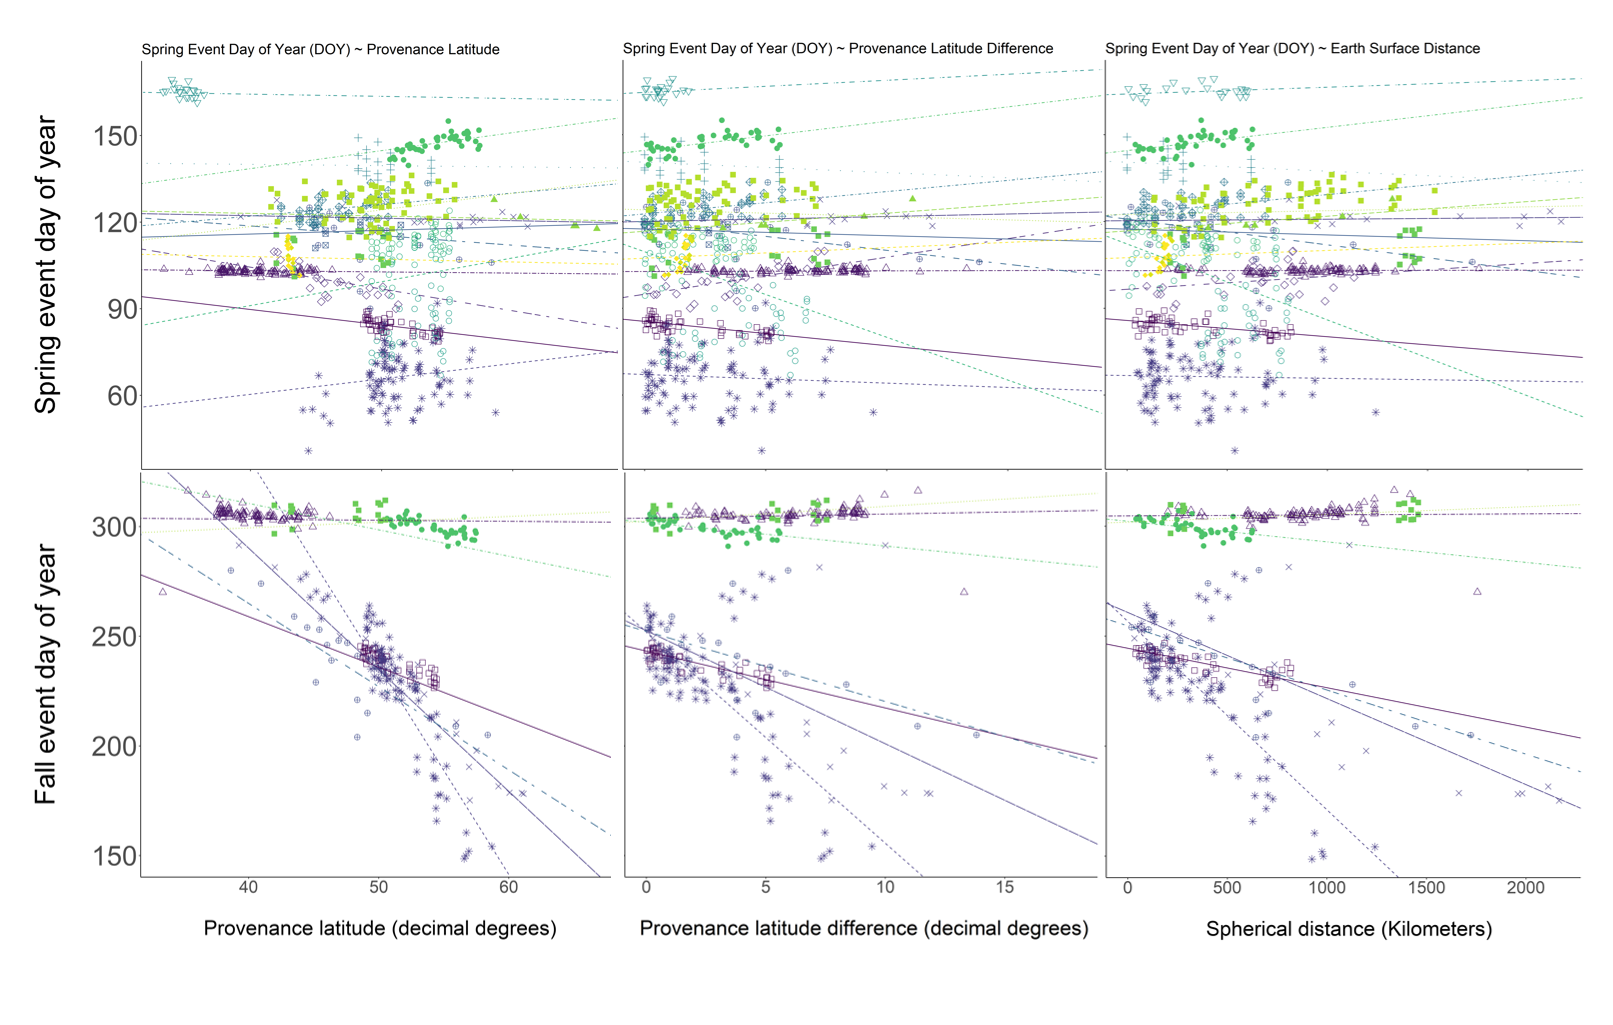
\includegraphics[width=\textwidth]{..//..//localadaptclim/Docs/figure_supp/lat_latdiff_earth_distance.jpg}
    \caption{Results were similar across different distance metrics: provenance latitude, difference between provenance and garden latitude, and spherical distance between provenance and garden.}
    \label{figure:lat_distance}
\end{figure}


\begin{figure}[!h] 
    \centering
 \includegraphics[width=\textwidth]{..//..//localadaptclim/Docs/figure_supp/overlap_scatterplot.jpg}
    \caption{Results from using climate overlap were not qualitatively different than using MAT.}
    \label{figure:overlap_scatterplot}
\end{figure}


\begin{figure}[!h] 
    \centering
 \includegraphics[width=\textwidth]{..//..//localadaptclim/Docs/figure_supp/overlap_posterior.jpg}
    \caption{We observed very weak effects of climate overlap on spring events (0.01 [0.02 - 0.03] days per one per cent increase in climate overlap), nearly identical across angiosperms (0.02 [0.00 - 0.05]) and gymnosperms (0.04 [0.00 - 0.09]). Fall events advanced as climate overlap declined, but slightly more strongly for gymnosperms
(advancing 0.72 [0.51 - 0.92] days per one per cent decline in climate overlap).}
    \label{figure:overlap_posterior}
\end{figure}



% \begin{figure}[!h] 
%     \centering
%  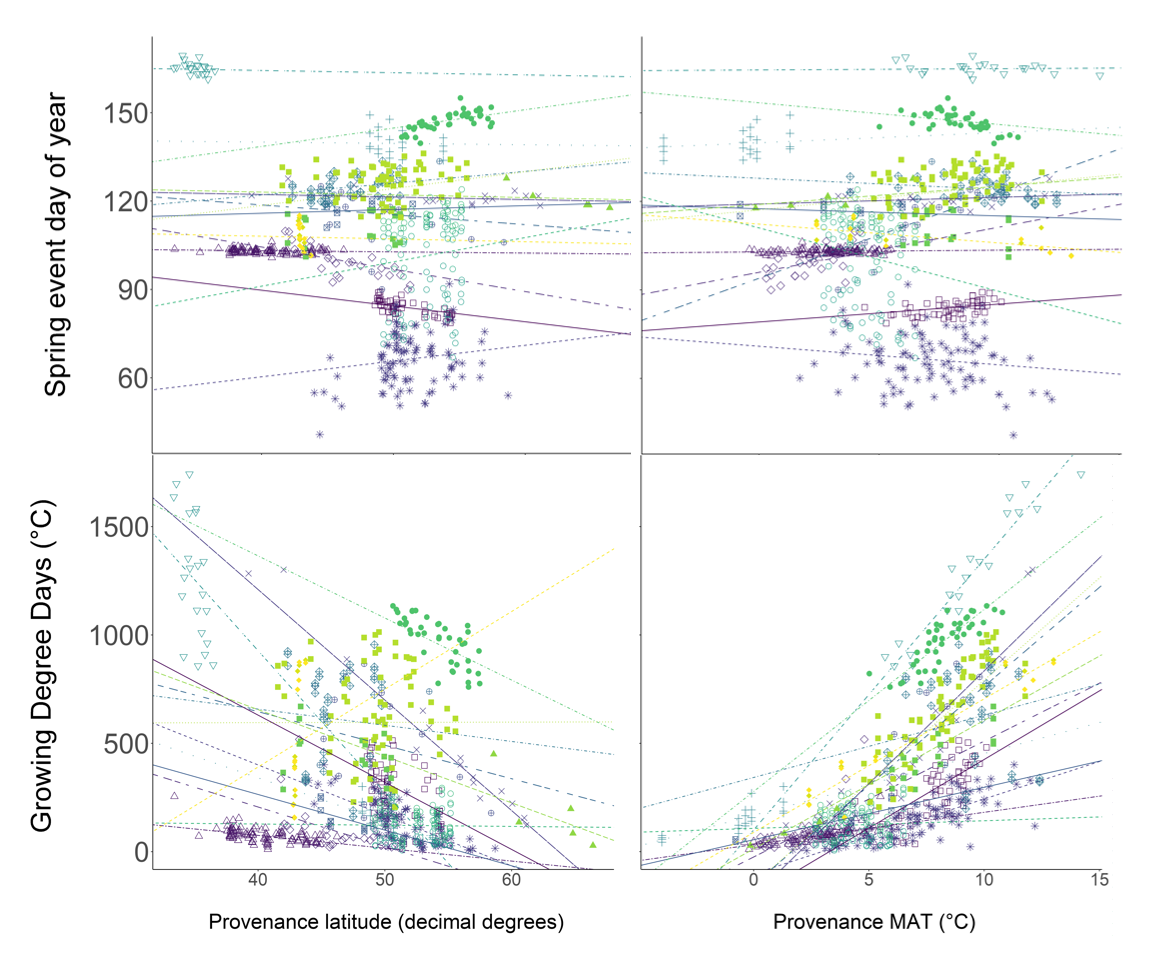
\includegraphics[width=\textwidth]{..//..//localadaptclim/Docs/figure_ms/gdd_ms.png}
%     \caption{Growing Degree Days (GDD)on each day of spring event in relation to provenance latitude and MAT, coded by symbol for species and color for garden with linear fits from hierarchical Bayesian models.}
%     \label{figure:gdd}
% \end{figure}

% 
% \begin{figure}[!h] 
%     \centering
%  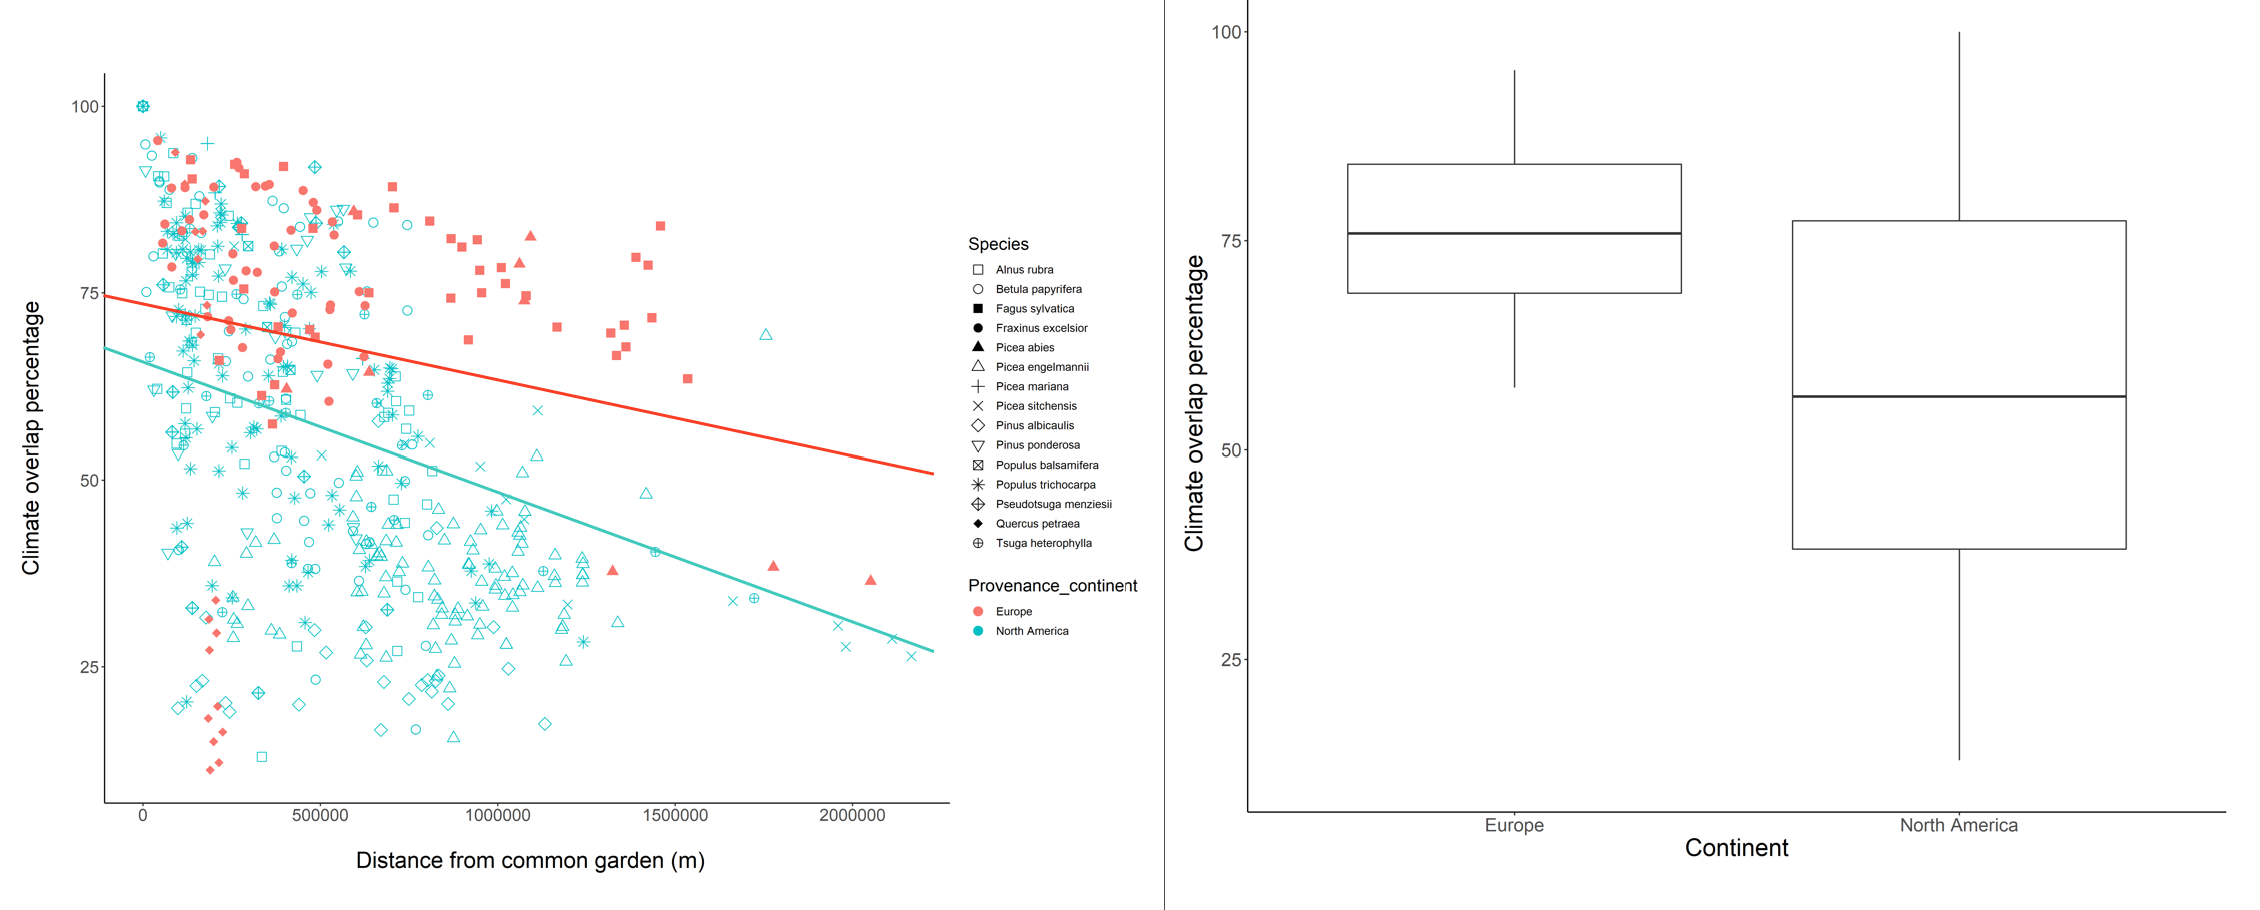
\includegraphics[width=\textwidth]{..//..//localadaptclim/Docs/figure_supp/climate_overlap_continent_comparison.png}
%     \caption{The closer a garden is to a provenance, the more overlap in temperature. 
% Higher extend of climate overlap in European studies.}
%     \label{figure:overlap_continent}
% \end{figure}
% 
% \begin{figure}[!h] 
%     \centering
%  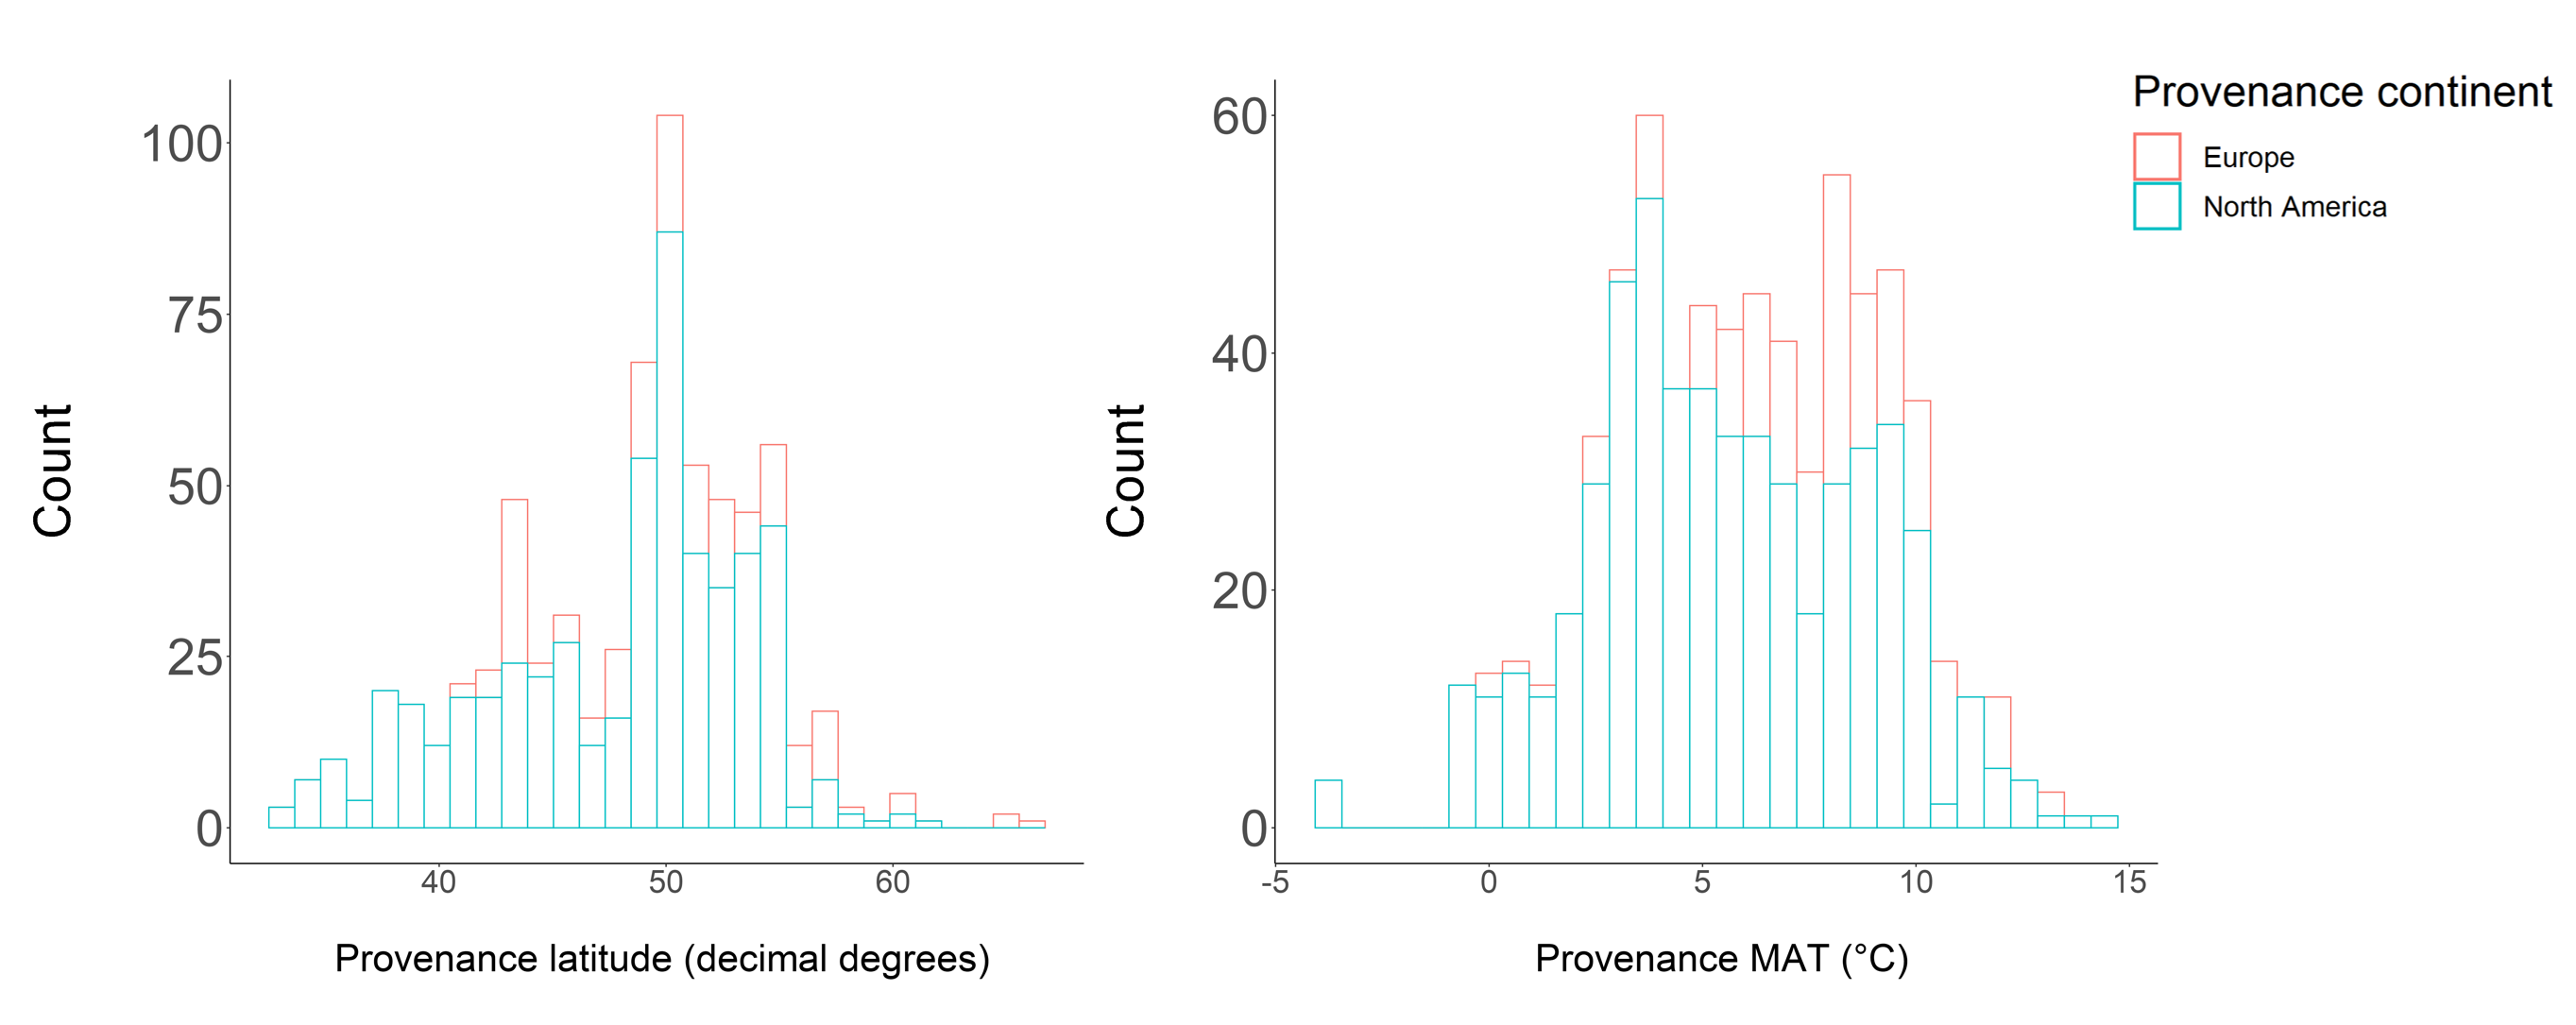
\includegraphics[width=\textwidth]{..//..//localadaptclim/Docs/figure_supp/prov_lat_mat_continent.png}
%     \caption{Placeholder.}
%     \label{figure:lat_mat_continent}
% \end{figure}
% 
% 
% \begin{figure}[!h] 
%     \centering
%  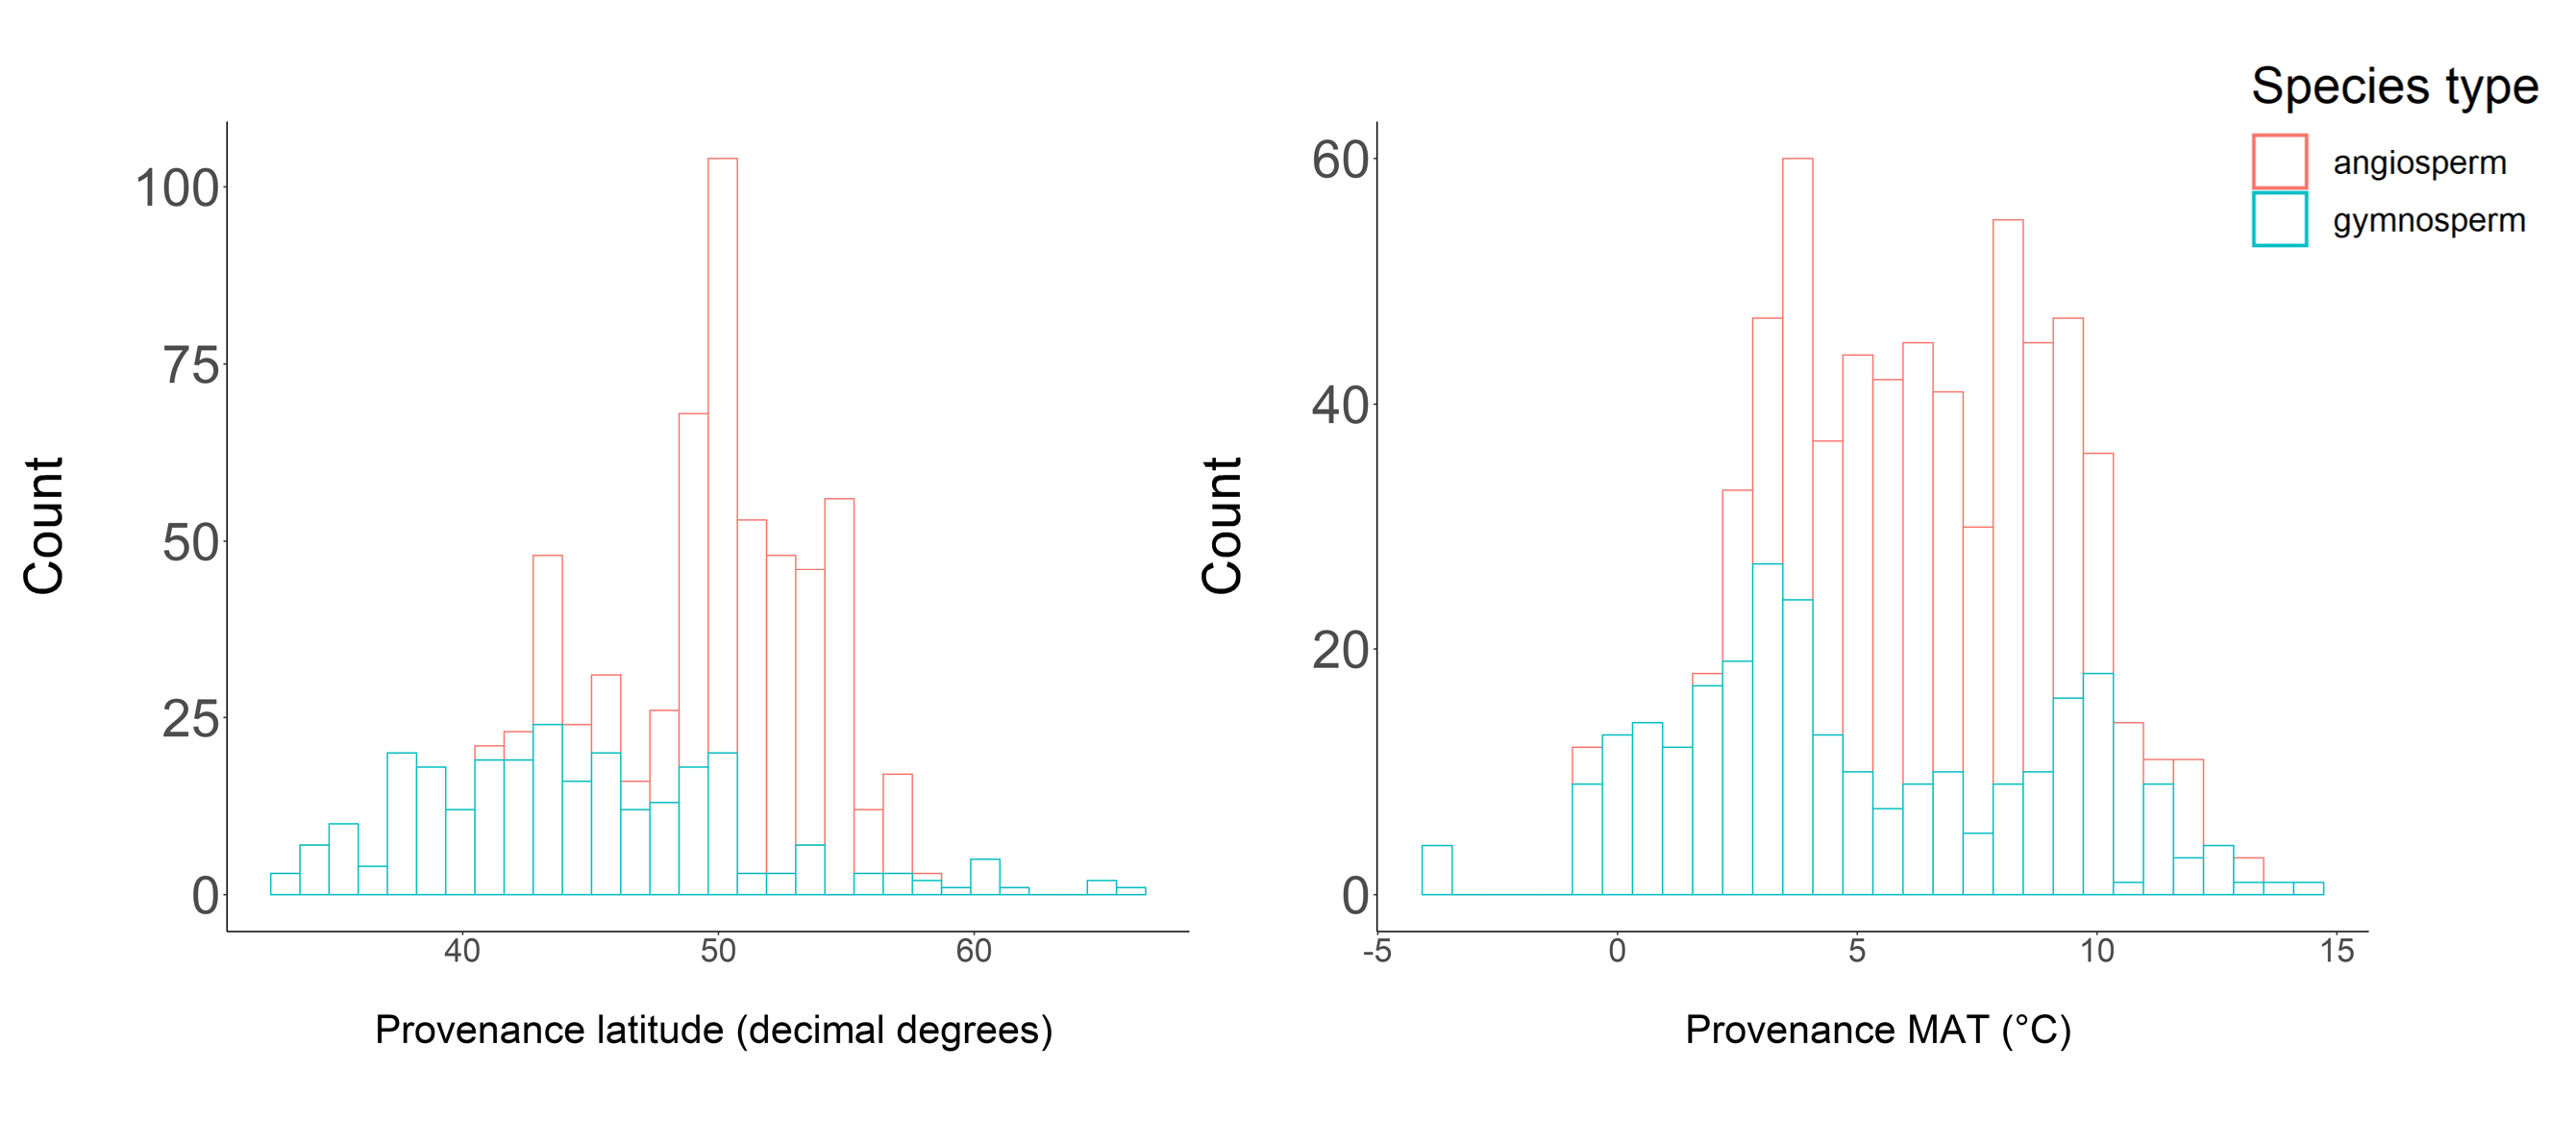
\includegraphics[width=\textwidth]{..//..//localadaptclim/Docs/figure_supp/spp_type_continent.png}
%     \caption{Placeholder}
%     \label{figure:spp_continent}
% \end{figure}
% 
 \end{document}
